\documentclass{standalone}
\usepackage{tikz}
\usetikzlibrary{patterns}
\usetikzlibrary{positioning}
\usetikzlibrary{patterns, positioning}
\usetikzlibrary{shapes.misc}
\usepackage[outline]{contour}
\contourlength{1.5pt} 
\usepackage[sfdefault]{ClearSans}

\begin{document}
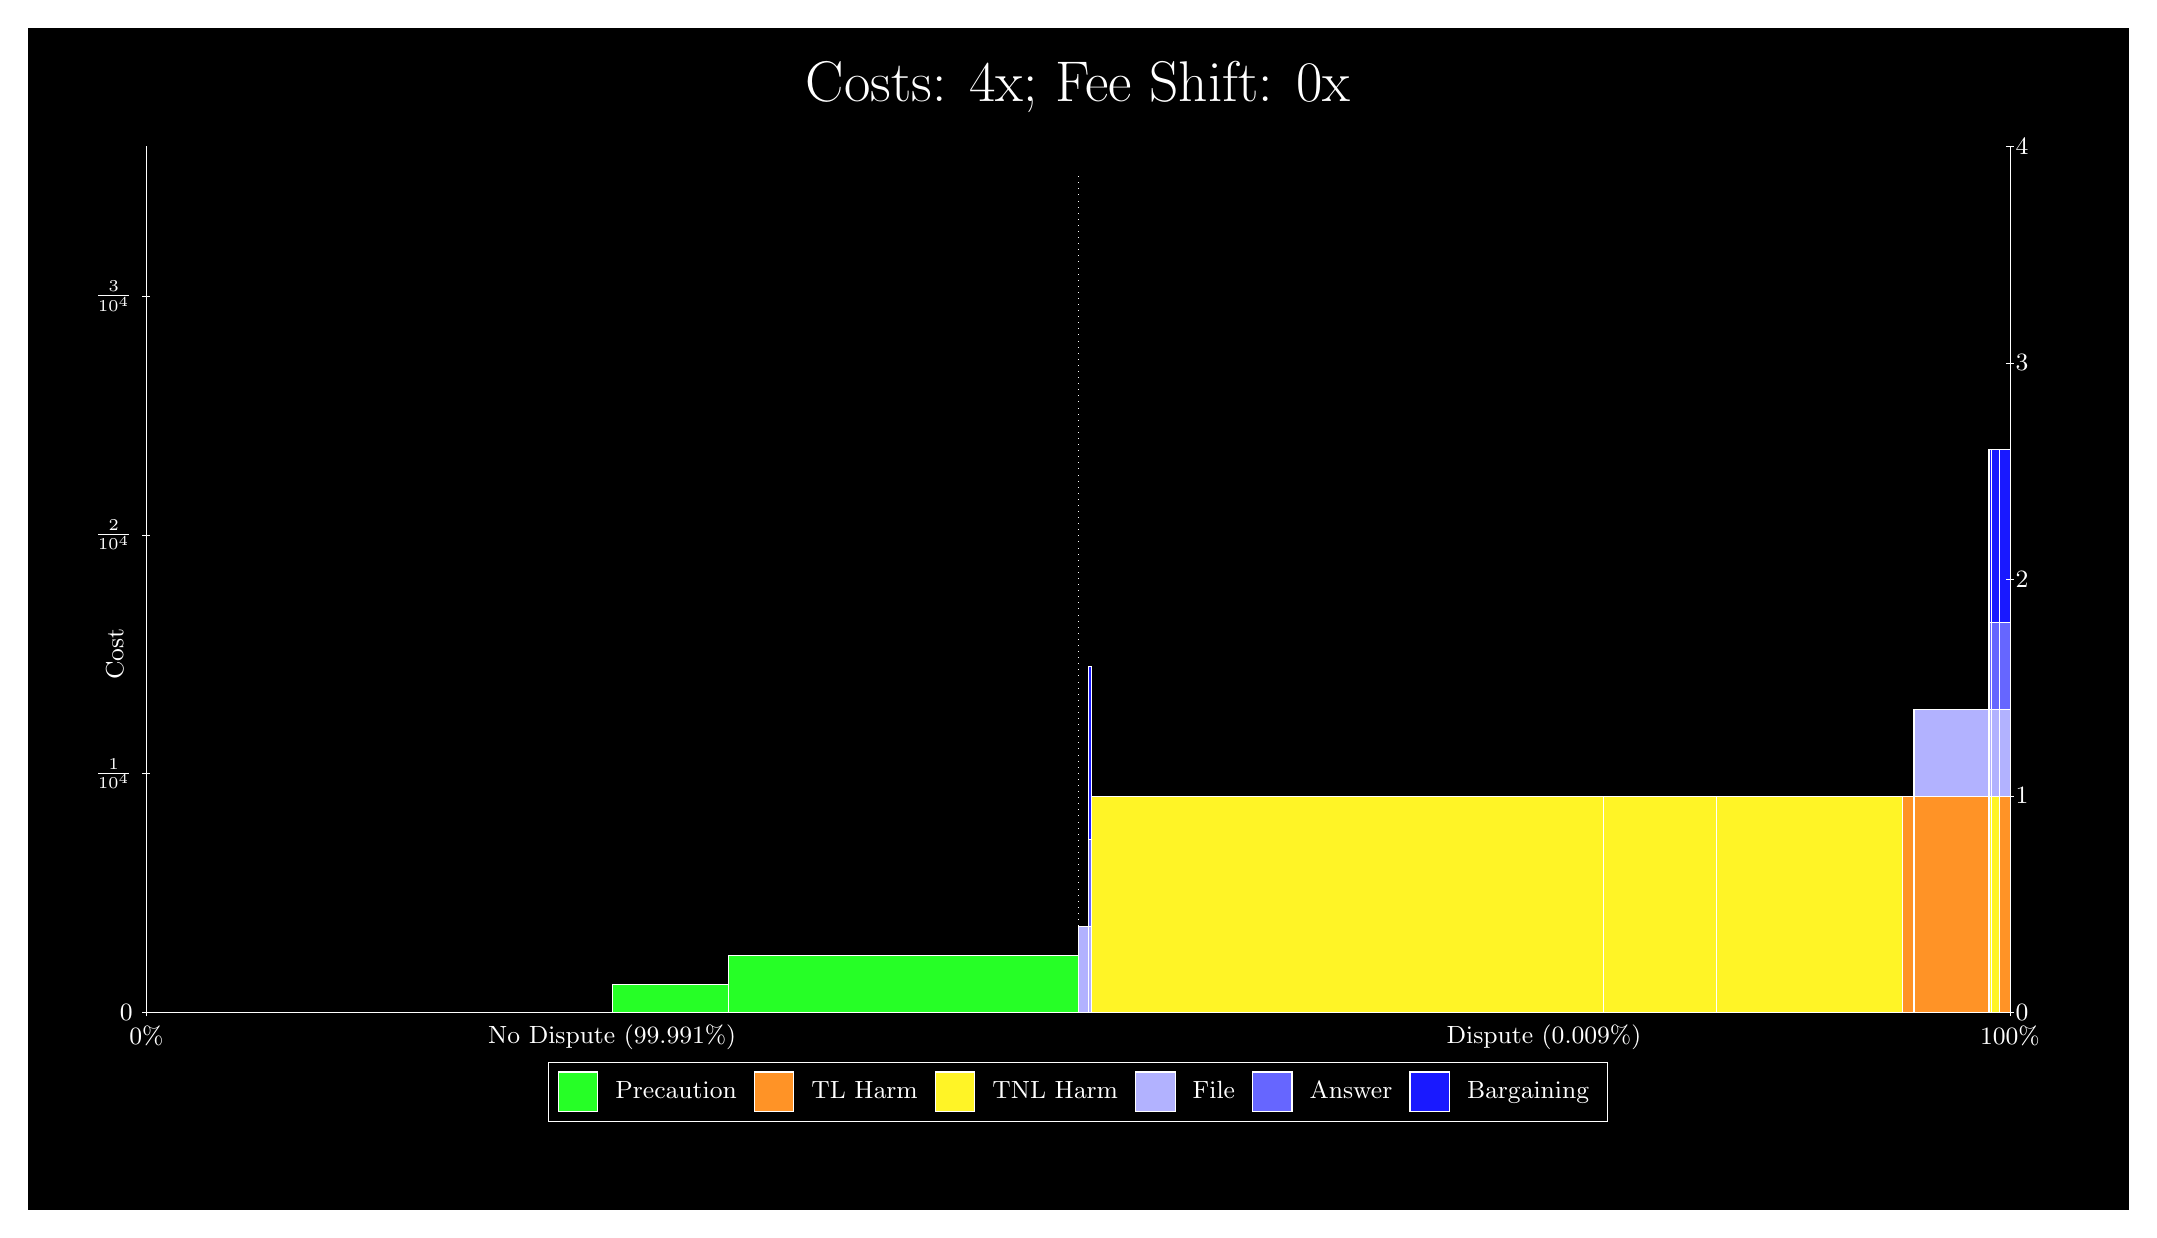
\begin{tikzpicture}
\draw[fill=black] (0,0) rectangle (26.667,15);
\draw[draw=none,text=white] (0,13.5) rectangle (26.667,15) node[midway] {\huge Costs: 4x; Fee Shift: 0x };
\draw[fill=green!85,draw=white,very thin] (7.4166,2.5) rectangle (8.8958,2.8639);
\draw[fill=green!85,draw=white,very thin] (8.8958,2.5) rectangle (13.333,3.2279);
\draw[fill=green!85,draw=white,very thin] (13.333,2.5) rectangle (13.462,2.5001);
\draw[fill=blue!30,draw=white,very thin] (13.333,2.5001) rectangle (13.462,3.6001);
\draw[fill=blue!30,draw=white,very thin] (13.462,2.5) rectangle (13.464,3.6);
\draw[fill=blue!60,draw=white,very thin] (13.462,3.6) rectangle (13.464,4.7);
\draw[fill=blue!90,draw=white,very thin] (13.462,4.7) rectangle (13.464,6.9);
\draw[fill=green!85,draw=white,very thin] (13.464,2.5) rectangle (13.466,2.5);
\draw[fill=blue!30,draw=white,very thin] (13.464,2.5) rectangle (13.466,3.6);
\draw[fill=blue!60,draw=white,very thin] (13.464,3.6) rectangle (13.466,4.7);
\draw[fill=blue!90,draw=white,very thin] (13.464,4.7) rectangle (13.466,6.9);
\draw[fill=green!85,draw=white,very thin] (13.466,2.5) rectangle (13.498,2.5001);
\draw[fill=blue!30,draw=white,very thin] (13.466,2.5001) rectangle (13.498,3.6001);
\draw[fill=blue!60,draw=white,very thin] (13.466,3.6001) rectangle (13.498,4.7001);
\draw[fill=blue!90,draw=white,very thin] (13.466,4.7001) rectangle (13.498,6.9001);
\draw[fill=yellow!85,draw=white,very thin] (13.498,2.5) rectangle (20.005,5.25);
\draw[fill=green!85,draw=white,very thin] (20.005,2.5) rectangle (21.442,2.5);
\draw[fill=yellow!85,draw=white,very thin] (20.005,2.5) rectangle (21.442,5.25);
\draw[fill=green!85,draw=white,very thin] (21.442,2.5) rectangle (23.801,2.5001);
\draw[fill=yellow!85,draw=white,very thin] (21.442,2.5001) rectangle (23.801,5.2501);
\draw[fill=green!85,draw=white,very thin] (23.801,2.5) rectangle (23.944,2.5001);
\draw[fill=orange!85,draw=white,very thin] (23.801,2.5001) rectangle (23.944,5.2501);
\draw[fill=green!85,draw=white,very thin] (23.944,2.5) rectangle (23.948,2.5001);
\draw[fill=yellow!85,draw=white,very thin] (23.944,2.5001) rectangle (23.948,5.2501);
\draw[fill=blue!30,draw=white,very thin] (23.944,5.2501) rectangle (23.948,6.3501);
\draw[fill=green!85,draw=white,very thin] (23.948,2.5) rectangle (24.891,2.5001);
\draw[fill=orange!85,draw=white,very thin] (23.948,2.5001) rectangle (24.891,5.2501);
\draw[fill=blue!30,draw=white,very thin] (23.948,5.2501) rectangle (24.891,6.3501);
\draw[fill=yellow!85,draw=white,very thin] (24.891,2.5) rectangle (24.909,5.25);
\draw[fill=blue!30,draw=white,very thin] (24.891,5.25) rectangle (24.909,6.35);
\draw[fill=blue!60,draw=white,very thin] (24.891,6.35) rectangle (24.909,7.45);
\draw[fill=blue!90,draw=white,very thin] (24.891,7.45) rectangle (24.909,9.65);
\draw[fill=green!85,draw=white,very thin] (24.909,2.5) rectangle (24.926,2.5);
\draw[fill=yellow!85,draw=white,very thin] (24.909,2.5) rectangle (24.926,5.25);
\draw[fill=blue!30,draw=white,very thin] (24.909,5.25) rectangle (24.926,6.35);
\draw[fill=blue!60,draw=white,very thin] (24.909,6.35) rectangle (24.926,7.45);
\draw[fill=blue!90,draw=white,very thin] (24.909,7.45) rectangle (24.926,9.65);
\draw[fill=green!85,draw=white,very thin] (24.926,2.5) rectangle (25.035,2.5001);
\draw[fill=yellow!85,draw=white,very thin] (24.926,2.5001) rectangle (25.035,5.2501);
\draw[fill=blue!30,draw=white,very thin] (24.926,5.2501) rectangle (25.035,6.3501);
\draw[fill=blue!60,draw=white,very thin] (24.926,6.3501) rectangle (25.035,7.4501);
\draw[fill=blue!90,draw=white,very thin] (24.926,7.4501) rectangle (25.035,9.6501);
\draw[fill=green!85,draw=white,very thin] (25.035,2.5) rectangle (25.167,2.5001);
\draw[fill=orange!85,draw=white,very thin] (25.035,2.5001) rectangle (25.167,5.2501);
\draw[fill=blue!30,draw=white,very thin] (25.035,5.2501) rectangle (25.167,6.3501);
\draw[fill=blue!60,draw=white,very thin] (25.035,6.3501) rectangle (25.167,7.4501);
\draw[fill=blue!90,draw=white,very thin] (25.035,7.4501) rectangle (25.167,9.6501);
\draw[white,very thin] (1.5,2.5) -- (1.5,13.5);
\node[font=\small,rotate=90,text=white, anchor=center] at (1.1, 7.0493) {Cost};
\draw[white,very thin] (1.45,2.5) -- (1.55,2.5);
\node[font=\small,text=white, anchor=east] at (1.45, 2.5) {0};
\draw[white,very thin] (1.45,5.5329) -- (1.55,5.5329);
\node[font=\small,text=white, anchor=east] at (1.45, 5.5329) {$\frac{1}{10^{4}}$};
\draw[white,very thin] (1.45,8.5658) -- (1.55,8.5658);
\node[font=\small,text=white, anchor=east] at (1.45, 8.5658) {$\frac{2}{10^{4}}$};
\draw[white,very thin] (1.45,11.599) -- (1.55,11.599);
\node[font=\small,text=white, anchor=east] at (1.45, 11.599) {$\frac{3}{10^{4}}$};

\draw[white,dotted,very thin] (13.333,2.83) -- (13.333,13.17);
\draw[white,very thin] (25.167,2.5) -- (25.167,13.5);
\draw[white,very thin] (25.117,2.5) -- (25.217,2.5);
\node[font=\small,text=white, anchor=west] at (25.117, 2.5) {0};
\draw[white,very thin] (25.117,5.25) -- (25.217,5.25);
\node[font=\small,text=white, anchor=west] at (25.117, 5.25) {1};
\draw[white,very thin] (25.117,8) -- (25.217,8);
\node[font=\small,text=white, anchor=west] at (25.117, 8) {2};
\draw[white,very thin] (25.117,10.75) -- (25.217,10.75);
\node[font=\small,text=white, anchor=west] at (25.117, 10.75) {3};
\draw[white,very thin] (25.117,13.5) -- (25.217,13.5);
\node[font=\small,text=white, anchor=west] at (25.117, 13.5) {4};

\draw[white,very thin] (1.5,2.5) -- (25.167,2.5);
\draw[white,very thin] (1.5,2.45) -- (1.5,2.55);
\node[font=\small,text=white, anchor=north] at (1.5, 2.45) {0\%};
\draw[white,very thin] (25.167,2.45) -- (25.167,2.55);
\node[font=\small,text=white, anchor=north] at (25.167, 2.45) {100\%};

\node[font=\small,text=white,anchor=south] at (7.4167, 1.9) {No\ Dispute\ (99.991\%)};
\node[font=\small,text=white,anchor=south] at (19.25, 1.9) {Dispute\ (0.009\%)};
\draw (13.3333,2.5) node (B) {};
\begin{scope}[align=center]
\matrix[scale=0.5,draw=white,below=0.5cm of B,nodes={draw},column sep=0.1cm]{
\node[rectangle,draw,minimum width=0.5cm,minimum height=0.5cm,fill=green!85]{}; & \node[draw=none,font=\small,text=white]{Precaution}; &
\node[rectangle,draw,minimum width=0.5cm,minimum height=0.5cm,fill=orange!85]{}; & \node[draw=none,font=\small,text=white]{TL Harm}; &
\node[rectangle,draw,minimum width=0.5cm,minimum height=0.5cm,fill=yellow!85]{}; & \node[draw=none,font=\small,text=white]{TNL Harm}; &
\node[rectangle,draw,minimum width=0.5cm,minimum height=0.5cm,fill=blue!30]{}; & \node[draw=none,font=\small,text=white]{File}; &
\node[rectangle,draw,minimum width=0.5cm,minimum height=0.5cm,fill=blue!60]{}; & \node[draw=none,font=\small,text=white]{Answer}; &
\node[rectangle,draw,minimum width=0.5cm,minimum height=0.5cm,fill=blue!90]{}; & \node[draw=none,font=\small,text=white]{Bargaining}; \\\\
};\end{scope}

\end{tikzpicture}
\end{document}